% Options for packages loaded elsewhere
% Options for packages loaded elsewhere
\PassOptionsToPackage{unicode}{hyperref}
\PassOptionsToPackage{hyphens}{url}
\PassOptionsToPackage{dvipsnames,svgnames,x11names}{xcolor}
%
\documentclass[
  letterpaper,
  DIV=11,
  numbers=noendperiod]{scrreprt}
\usepackage{xcolor}
\usepackage{amsmath,amssymb}
\setcounter{secnumdepth}{5}
\usepackage{iftex}
\ifPDFTeX
  \usepackage[T1]{fontenc}
  \usepackage[utf8]{inputenc}
  \usepackage{textcomp} % provide euro and other symbols
\else % if luatex or xetex
  \usepackage{unicode-math} % this also loads fontspec
  \defaultfontfeatures{Scale=MatchLowercase}
  \defaultfontfeatures[\rmfamily]{Ligatures=TeX,Scale=1}
\fi
\usepackage{lmodern}
\ifPDFTeX\else
  % xetex/luatex font selection
\fi
% Use upquote if available, for straight quotes in verbatim environments
\IfFileExists{upquote.sty}{\usepackage{upquote}}{}
\IfFileExists{microtype.sty}{% use microtype if available
  \usepackage[]{microtype}
  \UseMicrotypeSet[protrusion]{basicmath} % disable protrusion for tt fonts
}{}
\makeatletter
\@ifundefined{KOMAClassName}{% if non-KOMA class
  \IfFileExists{parskip.sty}{%
    \usepackage{parskip}
  }{% else
    \setlength{\parindent}{0pt}
    \setlength{\parskip}{6pt plus 2pt minus 1pt}}
}{% if KOMA class
  \KOMAoptions{parskip=half}}
\makeatother
% Make \paragraph and \subparagraph free-standing
\makeatletter
\ifx\paragraph\undefined\else
  \let\oldparagraph\paragraph
  \renewcommand{\paragraph}{
    \@ifstar
      \xxxParagraphStar
      \xxxParagraphNoStar
  }
  \newcommand{\xxxParagraphStar}[1]{\oldparagraph*{#1}\mbox{}}
  \newcommand{\xxxParagraphNoStar}[1]{\oldparagraph{#1}\mbox{}}
\fi
\ifx\subparagraph\undefined\else
  \let\oldsubparagraph\subparagraph
  \renewcommand{\subparagraph}{
    \@ifstar
      \xxxSubParagraphStar
      \xxxSubParagraphNoStar
  }
  \newcommand{\xxxSubParagraphStar}[1]{\oldsubparagraph*{#1}\mbox{}}
  \newcommand{\xxxSubParagraphNoStar}[1]{\oldsubparagraph{#1}\mbox{}}
\fi
\makeatother


\usepackage{longtable,booktabs,array}
\newcounter{none} % for unnumbered tables
\usepackage{calc} % for calculating minipage widths
% Correct order of tables after \paragraph or \subparagraph
\usepackage{etoolbox}
\makeatletter
\patchcmd\longtable{\par}{\if@noskipsec\mbox{}\fi\par}{}{}
\makeatother
% Allow footnotes in longtable head/foot
\IfFileExists{footnotehyper.sty}{\usepackage{footnotehyper}}{\usepackage{footnote}}
\makesavenoteenv{longtable}
\usepackage{graphicx}
\makeatletter
\newsavebox\pandoc@box
\newcommand*\pandocbounded[1]{% scales image to fit in text height/width
  \sbox\pandoc@box{#1}%
  \Gscale@div\@tempa{\textheight}{\dimexpr\ht\pandoc@box+\dp\pandoc@box\relax}%
  \Gscale@div\@tempb{\linewidth}{\wd\pandoc@box}%
  \ifdim\@tempb\p@<\@tempa\p@\let\@tempa\@tempb\fi% select the smaller of both
  \ifdim\@tempa\p@<\p@\scalebox{\@tempa}{\usebox\pandoc@box}%
  \else\usebox{\pandoc@box}%
  \fi%
}
% Set default figure placement to htbp
\def\fps@figure{htbp}
\makeatother





\setlength{\emergencystretch}{3em} % prevent overfull lines

\providecommand{\tightlist}{%
  \setlength{\itemsep}{0pt}\setlength{\parskip}{0pt}}



 


\KOMAoption{captions}{tableheading}
\makeatletter
\@ifpackageloaded{bookmark}{}{\usepackage{bookmark}}
\makeatother
\makeatletter
\@ifpackageloaded{caption}{}{\usepackage{caption}}
\AtBeginDocument{%
\ifdefined\contentsname
  \renewcommand*\contentsname{Table of contents}
\else
  \newcommand\contentsname{Table of contents}
\fi
\ifdefined\listfigurename
  \renewcommand*\listfigurename{List of Figures}
\else
  \newcommand\listfigurename{List of Figures}
\fi
\ifdefined\listtablename
  \renewcommand*\listtablename{List of Tables}
\else
  \newcommand\listtablename{List of Tables}
\fi
\ifdefined\figurename
  \renewcommand*\figurename{Figure}
\else
  \newcommand\figurename{Figure}
\fi
\ifdefined\tablename
  \renewcommand*\tablename{Table}
\else
  \newcommand\tablename{Table}
\fi
}
\@ifpackageloaded{float}{}{\usepackage{float}}
\floatstyle{ruled}
\@ifundefined{c@chapter}{\newfloat{codelisting}{h}{lop}}{\newfloat{codelisting}{h}{lop}[chapter]}
\floatname{codelisting}{Listing}
\newcommand*\listoflistings{\listof{codelisting}{List of Listings}}
\makeatother
\makeatletter
\makeatother
\makeatletter
\@ifpackageloaded{caption}{}{\usepackage{caption}}
\@ifpackageloaded{subcaption}{}{\usepackage{subcaption}}
\makeatother
\usepackage{bookmark}
\IfFileExists{xurl.sty}{\usepackage{xurl}}{} % add URL line breaks if available
\urlstyle{same}
\hypersetup{
  pdftitle={Mathematical Foundations for Economics Students},
  pdfauthor={Isabella García},
  colorlinks=true,
  linkcolor={blue},
  filecolor={Maroon},
  citecolor={Blue},
  urlcolor={Blue},
  pdfcreator={LaTeX via pandoc}}


\title{Mathematical Foundations for Economics Students}
\author{Isabella García}
\date{2026-07-01}
\begin{document}
\maketitle

\renewcommand*\contentsname{Table of contents}
{
\setcounter{tocdepth}{2}
\tableofcontents
}

\bookmarksetup{startatroot}

\chapter*{Preface}\label{preface}
\addcontentsline{toc}{chapter}{Preface}

\markboth{Preface}{Preface}

This website is a development in progress to serve as an open-access
mathematical compendium covering mathematical topics fundamental for any
student of economics.

Version 0.0 of this resource is to include Trigonometry, Calculus I,
Calculus II, and applications of such topics in the context of
Economics.

This resource is designed for long-term expansion across additional,
related subjects that will build upon the necessary, basic principles
that Version 0.0 introduces.

Since this is an independent project that is following concurrently with
my own studies, I'd like to ask that you please pardon the ongoing
construction. All errors are my own.

\part{Trigonometry}

\chapter{Basics of Trigonometry}\label{basics-of-trigonometry}

\section{The Three Primary Functions}\label{the-three-primary-functions}

In mathematics, there are six fundamental trigonometric functions. For
simplicity, we will begin with the three primary functions to establish
the basic framework and then introduce their reciprocals later on. The
three primary functions are as follows with their classic mnemonic for
easy recall. \[
\begin{array}{ccc}
\textbf{SOH} & \textbf{CAH} & \textbf{TOA} \\[6pt]
\sin\theta = \dfrac{\text{opp}}{\text{hyp}} &
\cos\theta = \dfrac{\text{adj}}{\text{hyp}} &
\tan\theta = \dfrac{\text{opp}}{\text{adj}}
\end{array}
\]

Sine, cosine, and tangent compare the angles of a right triangle to the
ratios of its side lengths. The pythagorean theorem,
\(a^2 + b^2 = c^2\), finds missing sides of a right triangle, with \(a\)
being the side opposite from the angle, \(b\) being the side next to the
angle, and \(c\) being the hypotenuse, or the longest side. Because of
this connection, we can similarly write the three primary functions as:
\[
\sin\theta = \frac{a}{c} \qquad
\cos\theta = \frac{b}{c} \qquad
\tan\theta = \frac{a}{b}
\]

\pandocbounded{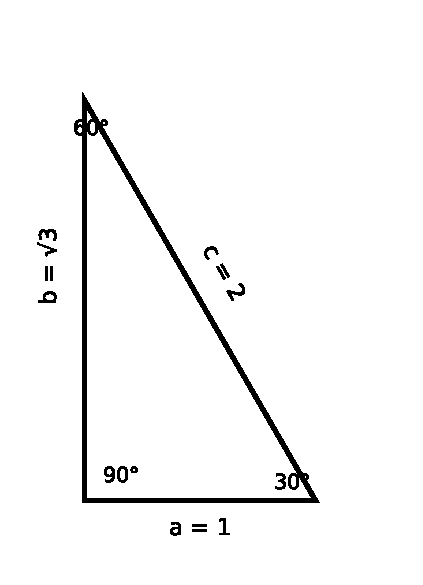
\includegraphics[keepaspectratio]{trig/basics_files/figure-pdf/cell-2-output-1.pdf}}

\section{The Unit Circle}\label{the-unit-circle}

The \textbf{unit circle} is a circle of radius \(r = 1\) centered at the
origin of the Cartesian plane. It is the foundation of trigonometry and,
by extension, of much of calculus.

For any angle \(\theta\) measured counterclockwise from the positive
\(x\)-axis, the corresponding point on the unit circle is:

\[
(\cos\theta,\ \sin\theta)
\]

\chapter{Trigonometric Identities}\label{trigonometric-identities}

\chapter{Inverse Trigonometric
Functions}\label{inverse-trigonometric-functions}

\part{Calculus I}

\chapter{Derivatives}\label{derivatives}

\part{Calculus II}

\chapter{Integration Techniques}\label{integration-techniques}

\part{Mathematical Economics}

\chapter{Optimization}\label{optimization}

\chapter{Supply and Demand}\label{supply-and-demand}




\end{document}
